\begin{figure}[H]
\centering
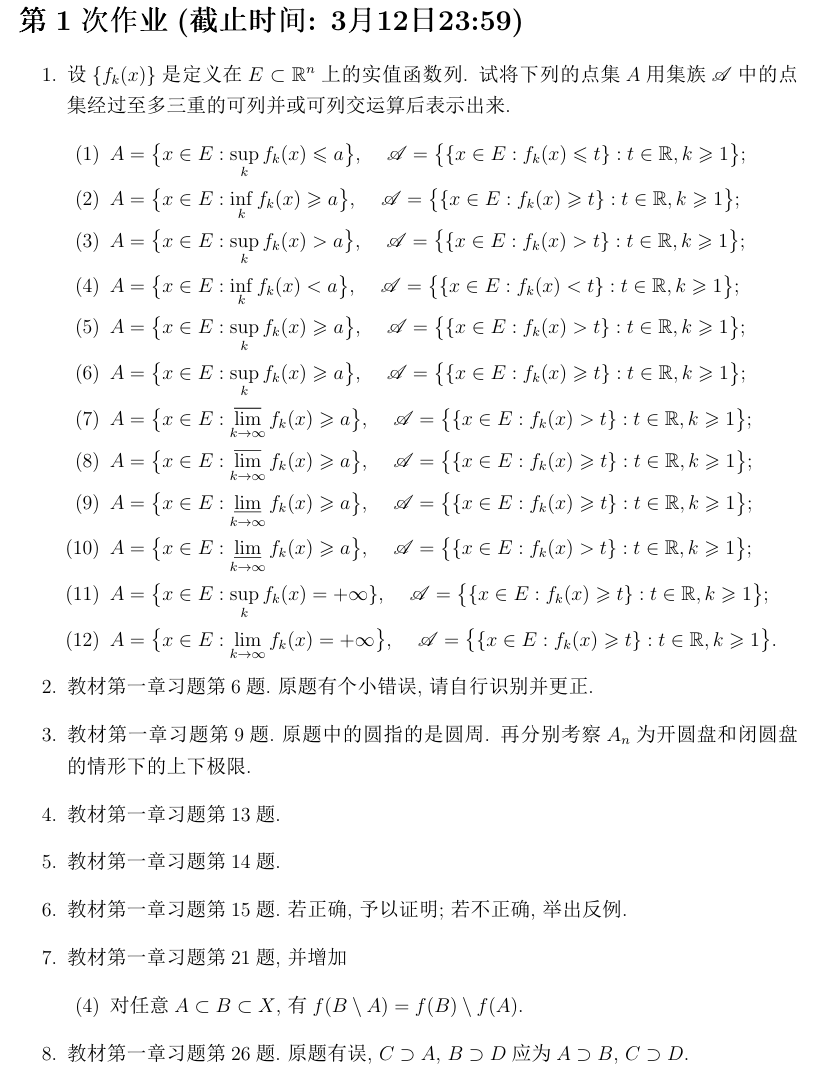
\includegraphics[width=\textwidth]{hw1-20250307.png}
% \caption{}
\label{}
\end{figure}

(1)
\[
A=\{ x\in E :\sup_{k}f_k(x)\leq a\} =\bigcap_{k=1}^{\infty}\{ x\in E:f_k(x)\leq a \}
\]
(2)
\[
A=\{ x\in E:\inf _kf_k(x)\geq a \}=\bigcup_{k=1}^{\infty}\left\{  x\in E :f_k(x)\geq a \right\}
\]
(3) take completion of both side of (1)
\[
A=\{ x\in E :\sup _kf_k(x)>a\}=A_1^{c}=\left( \bigcap_{k=1}^{\infty}  \{ x\in E:f_k(x)\leq a \}\right)^{c}=\bigcup_{k=1}^{\infty} \{ x\in E:f_k(x)>a \}
\]
(4) take completion of both side of (2)
\[
A=\{ x\in E:\inf _kf_k(x)<a\}=A_2^{c}=\left( \bigcup_{k=1}^{\infty} \{ x\in E :f_k(x)<a\} \right)^{c}=\bigcup_{k=1}^{\infty} \{ x\in E:f_k(x)<a \}
\]
(5) for any $x\in A$, $\sup _kf_k(x)\geq a$ means that for any $\epsilon>0$, there exists a $k$ such that $f_k(x)>a-\epsilon$. In the set language,
\[
A=\{ x\in E:\sup _kf_k(x)\geq a \}=\bigcap_{n=1}^{\infty}\bigcup_{k=1}^{\infty} \left\{  x\in E:f_k(x)>a-\frac{1}{n}  \right\}
\]
(6) for any $x\in A$, $\sup _kf_k(x)\geq a$ means that for any $\epsilon>0$, there exists a $k$ such that $f_k(x)\geq a-\epsilon$. In the set language,
\[
A=\{ x\in E:\sup _kf_k(x)\geq a \}=\bigcap_{n=1}^{\infty}\bigcup_{k=1}^{\infty} \left\{  x\in E:f_k(x)\geq  a-\frac{1}{n}  \right\}
\]
(7) combining with the result in (2) and (5) yields
\[
\left\{x \in E: \varlimsup_{k \rightarrow \infty} f_k(x) \geqslant a\right\}=\bigcap_{i=1}^{\infty} \bigcap_{j=1}^{\infty} \bigcup_{k=j}^{\infty}\left\{x \in E: f_k(x)>a-\frac{1}{i}\right\} ;
\]
(8) similar to (7)
\[
\left\{x \in E: \varlimsup_{k \rightarrow \infty} f_k(x) \geqslant a\right\}=\bigcap_{i=1}^{\infty} \bigcap_{j=1}^{\infty} \bigcup_{k=j}^{\infty}\left\{x \in E: f_k(x) \geqslant a-\frac{1}{i}\right\} ;
\]
(9)
\[
\begin{aligned}
\{ x\in E:\liminf_{ k \to \infty } f_k(x)\geq a \} & =\{ x\in E:\lim_{ n \to \infty } \inf_{k\geq n}f_k(x)\geq a \} \\
 & \eqqcolon \{ x\in E:\lim_{ n \to \infty } g_n(x)\geq a \} \\
 & =\bigcap_{m=1}^{\infty} \bigcup_{n=1}^{\infty}\left\{  x\in E:\inf_{k\geq n}f_k(x)\geq a-\frac{1}{m}  \right\} \\
 & =\bigcap_{m=1}^{\infty} \bigcup_{n=1}^{\infty} \bigcap_{k=n}^{\infty }\left\{  x\in E:f_k(x)\geq a-\frac{1}{m}  \right\}  
\end{aligned}
\]
(10) similar to (9)
\[
\{ x\in R:\liminf_{ k \to \infty } f_k(x)\geq a \}=\bigcap_{m=1}^{\infty}\bigcup_{n=1}^{\infty} \bigcap_{k=n}^{\infty} \left\{  x\in E:f_k(x)>a-\frac{1}{m}  \right\}
\]
(11)
\[
\begin{aligned}
\{ x\in R:\sup _kf_k(x)=+\infty \} & =\bigcap_{m=1}^{\infty} \{ x\in R:\sup _kf_k(x)\geq m \} \\
 & \overset{ (6) }{ = }\bigcap_{m=1}^{\infty} \bigcap_{n=1}^{\infty} \bigcup_{k=1}^{\infty} \left\{  x\in E:f(x)\geq m-\frac{1}{n}  \right\} \\
 & =\bigcap_{m=1}^{\infty} \bigcup_{k=1}^{\infty} \{ x\in E:f(x)\geq m \}
\end{aligned}
\]
(12) Since $\left\{x \in E: \lim _{k \rightarrow \infty} f_k(x)=+\infty\right\}=\left\{x \in E: \varliminf_{k \rightarrow \infty} f_k(x)=+\infty\right\}=\{x \in E$: $\left.\sup _j \inf _{k \geqslant j} f_k(x)=+\infty\right\}$, combining with the results of $(11)(2)$ yields the desired conclusion.
\[
\left\{x \in E: \lim _{k \rightarrow \infty} f_k(x)=+\infty\right\}=\bigcap_{i=1}^{\infty} \bigcup_{j=1}^{\infty} \bigcap_{k=j}^{\infty}\left\{x \in E: f_k(x) \geqslant i\right\} .
\]
\begin{figure}[H]
\centering
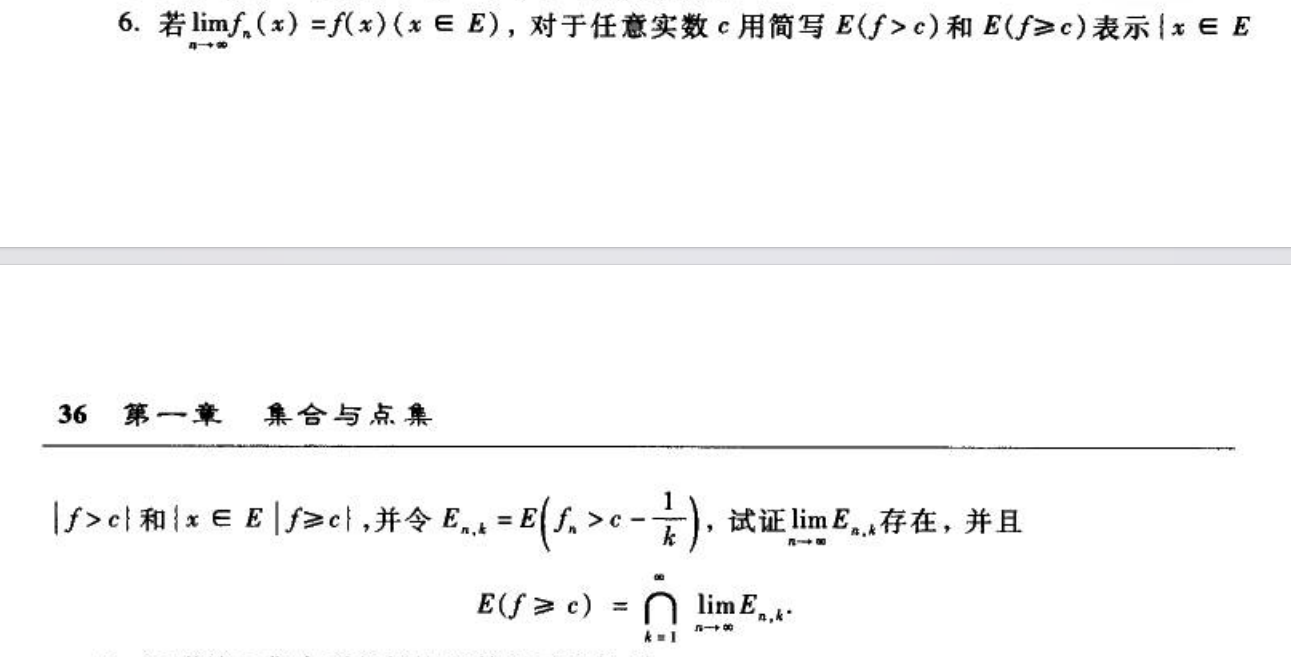
\includegraphics[width=\textwidth]{1-hw1-20250307.png}
% \caption{}
\label{}
\end{figure}
Find an error of the question above.

Errata:
If $\lim_{ n \to \infty }f_n(x)=f(x)$ for $x\in E$, $E_{n,k}\coloneqq \left\{  x\in E:f_n(x)>c-\frac{1}{k}  \right\}$, show that for each fixed $k$, $\lim_{ n \to \infty }E_{n,k}$ exists and
\[
\{ x\in E:f(x)\geq c \}=\bigcap_{k=1}^{\infty}\lim_{ n \to \infty } E_{n,k}
\]
Fix $k$ then $\lim_{ n \to \infty }E_{n,k}$ exists iff $\limsup_{ n \to \infty }E_{n,k}$ and $\liminf_{ n \to \infty }E_{n,k}$ exists and equals.
\[
\limsup_{ n \to \infty } E_{n,k}=\bigcap_{m=1}^{\infty}\bigcup_{n=m}^{\infty} E_{n,k}= \bigcap_{m=1}^{\infty}\bigcup_{n=m}^{\infty} \left\{  x\in E:f_n(x)>c-\frac{1}{k}  \right\}=\left\{  x\in E:\limsup_{ n \to \infty } f_n(x)>c-\frac{1}{k}  \right\}
\]
\[
\liminf_{ n \to \infty } E_{n,k}=\left\{  x\in E:\liminf_{ n \to \infty } f_n(x)>c-\frac{1}{k}  \right\}
\]
Since $\lim_{ n \to \infty }f_n(x)=f(x)$ exists, $\limsup_{ n \to \infty }f_n(x)=\liminf_{ n \to \infty }f_n(x)$ thus $\limsup_{ n \to \infty }E_{n,k}=\liminf_{ n \to \infty }E_{n,k}$. Hence $\lim_{ n \to \infty }E_{n,k}$ exists and equals to $\left\{   x\in E:f(x)>c-\frac{1}{k}  \right\}$. Obviously, $\{ x\in E:f(x)\geq c \}=\bigcap_{k=1}^{\infty}\lim_{ n \to \infty }E_{n,k}$.

\begin{figure}[H]
\centering
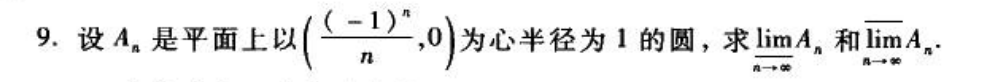
\includegraphics[width=\textwidth]{2-hw1-20250307.png}
% \caption{}
\label{}
\end{figure}
\[
A_n=\left\{  (x,y):\left( x-\frac{(-1)^{n}}{n} \right)^{2}+y^{2}= 1  \right\}
\]
Then
\[
\liminf_{ n \to \infty } A_n=\bigcup_{n=1}^{\infty} \bigcap_{k=n}^{\infty}A_k=\bigcup_{n=1}^{\infty} (\varnothing)=\varnothing
\]
\[
\limsup_{ n \to \infty } A_n=\bigcap_{n=1}^{\infty} \bigcup_{k=n}^{\infty} A_k=\{ (x,y)\in \mathbb{R}^{2}: \exists \text{ infinite many }k_j\text{ such that } (x,y)\in A_{k_j}\}
\]
If $(x, y)\in A_m\cap A_n,m\neq n$ then $(x, y)\not\in A_k$ for $k\neq m,k\neq n$. Therefore $\limsup_{ n \to \infty }A_n=\varnothing$.

For
\[
A_n=\left\{  (x,y):\left( x-\frac{(-1)^{n}}{n} \right)^{2}+y^{2}\leq   1  \right\}
\]
Then
\[
\liminf_{ n \to \infty }A_n=\{ (x,y)\in \mathbb{R}^{2}: \exists K,\text{s.t. }(x,y)\in A_k\text{ for all }k>K \}
\]
\[
\limsup_{ n \to \infty } A_n=\{(x,y)\in \mathbb{R}^{2}: \exists \text{ infinite many }k_j\text{ such that } (x,y)\in A_{k_j}\}
\]
Claim that
\[
\liminf_{ n \to \infty }A_n = \{ (x,y):x^{2}+y^{2}<1 \}
\]
\[
\limsup_{ n \to \infty } A_n=\{ (x, y):x^{2}+y^{2}\leq1 \}\setminus \{ (0,1),(0,-1) \}
\]
For
\[
A_n=\left\{  (x,y):\left( x-\frac{(-1)^{n}}{n} \right)^{2}+y^{2}<   1  \right\}
\]
Then
\[
\liminf_{ n \to \infty }A_n=\{ (x,y)\in \mathbb{R}^{2}: \exists K,\text{s.t. }x\in A_k\text{ for all }k>K \}
\]
\[
\limsup_{ n \to \infty } A_n=\{(x,y)\in \mathbb{R}^{2}: \exists \text{ infinite many }k_j\text{ such that } (x,y)\in A_{k_j}\}
\]
Claim that
\[
\liminf_{ n \to \infty }A_n = \{ (x,y):x^{2}+y^{2}<1 \}
\]
\[
\limsup_{ n \to \infty } A_n=\{ (x, y):x^{2}+y^{2}\leq1 \}\setminus \{ (0,1),(0,-1) \}
\]
\begin{figure}[H]
\centering
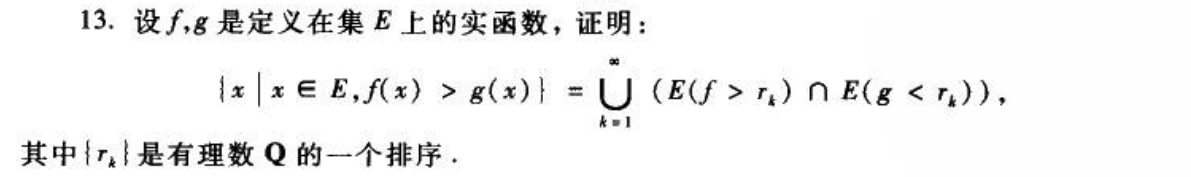
\includegraphics[width=\textwidth]{3-hw1-20250307.png}
% \caption{}
\label{}
\end{figure}

Denote that
\[
A=\{ x\in E:f(x)>g(x) \},\quad B=\bigcup_{k=1}^{\infty} (\{ x\in E :f(x)>r_k\}\cap \{ x\in E:g(x)<r_k \})
\]
For $x\in A$, we have $f(x)>g(x)$. Since $\mathbb{Q}$ is dense in $\mathbb{R}$, there exists $r_k\in(g(x),f(x))$ for some $k$, thus $x\in \{ x\in E:f(x)>r_k \}\cap \{ x\in E :g(x)<r_k\}\subset B$. Therefore $A\subset B$.

For $x\in B$, we have $f(x)>r_k,g(x)<r_k$ for some $k$ then $f(x)<g(x)$, i.e. $x\in \{ x\in E:f(x)>g(x)\}$. Therefore $A\supset B$. Hence $A=B$.

\begin{figure}[H]
\centering
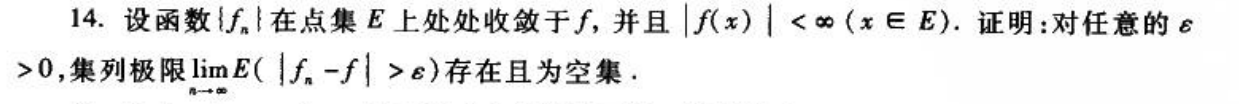
\includegraphics[width=\textwidth]{4-hw1-20250307.png}
% \caption{}
\label{}
\end{figure}

For any $\epsilon>0$, denote that
\[
A_n=\{ x\in E:\lvert f_n(x)-f(x) \rvert >\epsilon \}
\]
Since $f_n\to f$ on $E$ pointwisely and $\lvert f (x) \rvert<\infty,\forall x\in E$ ,we know that for any fixed $x\in E$, we have $\lim_{ n \to \infty }f_n(x)=f(x)$ i.e. there exists $N>0$ such that $\lvert f_n(x)-f(x) \rvert<\epsilon$ for all $n>N$.
\[
\liminf_{ n \to \infty }A_n=\{ x\in E: \exists K,\text{s.t. }x\in A_k\text{ for all }k>K \}=\varnothing
\]
\[
\limsup_{ n \to \infty } A_n=\{x\in E: \exists \text{ infinite many }k_j\text{ such that } x\in A_{k_j}\}=\varnothing
\]
Therefore $\lim_{ n \to \infty }A_n$ exists and equals to $\varnothing$.

\begin{figure}[H]
\centering
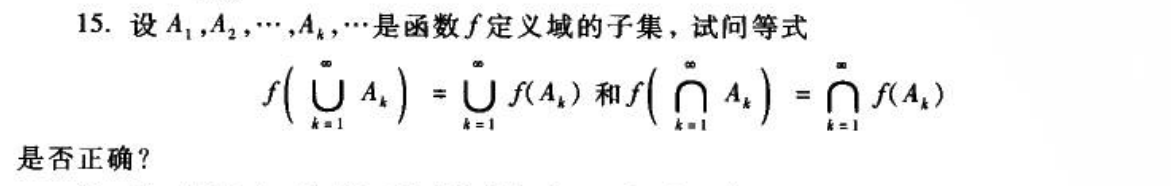
\includegraphics[width=\textwidth]{5-hw1-20250307.png}
% \caption{}
\label{}
\end{figure}
\[
f\left( \bigcup_{k=1}^{\infty} A_k \right)=\bigcup_{k=1}^{\infty} f(A_k)\qquad f\left( \bigcap_{k=1}^{\infty} A_k \right)\subset \bigcap_{k=1}^{\infty} f(A_k)
\]
Since $A_k\subset \bigcup_{k=1}^{\infty}A_k$ for any $k$, $f(A_k)\subset f\left( \bigcup_{k=1}^{\infty}A_k \right)$. Therefore $\bigcup_{k=1}^{\infty}f(A_k)\subset f\left( \bigcup_{k=1}^{\infty}A_k \right)$.

If $x\in f\left( \bigcup_{k=1}^{\infty} A_k\right)=\left\{  f(y):y\in \bigcup_{k=1}^{\infty}A_k  \right\}$, then there exists $y\in \bigcup_{k=1}^{\infty}A_k$ such that $f(y)=x$. By the definition of $\bigcup_{k=1}^{\infty}$, we have $y\in A_n$ for some $n\in \mathbb{N}$ thus $x\in f(A_n)\subset \bigcup_{k=1}^{\infty}f(A_k)$. Therefore $f\left( \bigcup_{k=1}^{\infty}A_k \right)\subset \bigcup_{k=1}^{\infty}f(A_k)$. Hence $f\left( \bigcup_{k=1}^{\infty}A_k \right)=\bigcup_{k=1}^{\infty}f(A_k)$.

For $x\in f\left( \bigcap_{k=1}^{\infty}A_k \right)$, there exists $y\in \bigcap_{k=1}^{\infty}A_k$ such that $x=f(y)$. For any $n\in \mathbb{N}$, $y\in \bigcap_{k=1}^{\infty}A_k\subset A_n$ then $x\in f(A_n)$. Therefore $x\in \bigcap_{k=1}^{\infty }f(A_k)$, i.e. $f\left( \bigcap_{k=1}^{\infty} f(A_k)\right)\subset \bigcap_{k=1}^{\infty}f(A_k)$.

\begin{figure}[H]
\centering
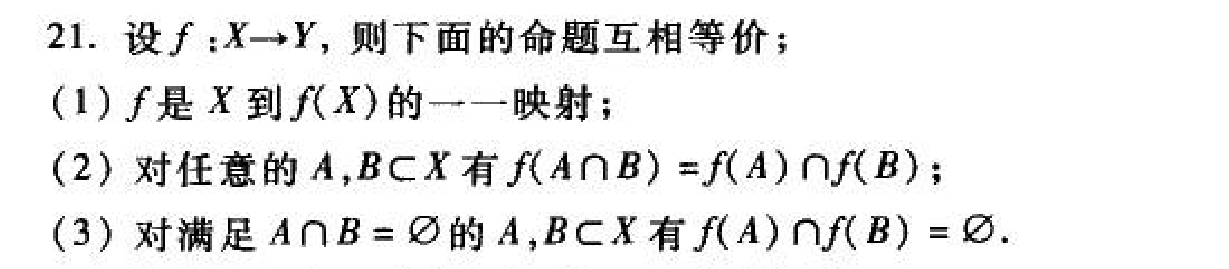
\includegraphics[width=\textwidth]{6-hw1-20250307.png}
% \caption{}
\label{}
\end{figure}

(4) 对任意 $A\subset B\subset X$ 有 $f (B\setminus A)=f (B)\setminus f(A)$.

(1) means $f$ is one-one. Since $f:X\to f(X)$ is defined to be onto, then (1) means if $x\neq y$ for $x, y\in X$ then $f(x)\neq f(y)$. In other words, if $f(x)=f(y)$ then $x=y$.

(1)=>(2): for any $x\in A\cap B$, we have $x\in A$ and $x\in B$ then $f (x)\in f(A)$ and $f (x)\in f(B)$ thus $x\in f(A)\cap f(B)$. Therefore $f(A\cap B)\subset f(A)\cap f(B)$.

It suffices to show that $f(A)\cap f(B)\subset f(A\cap B)$. We argue by contradiction. If there is an element $y\in f(A)\cap f(B)$ not containd in $f(A\cap B)$, then there exists $a\in A$ and $b\in B$ such that $f(a)=y$, $f(b)=y$. Since $f$ is one-one, we have $a=b$. Therefore $a=b\in A\cap B$, $y=f (a)\in f(A\cap B)$, which is a contradiction. Hence $f(A)\cap f(B)\subset f(A\cap B)\Rightarrow f(A)\cap f(B)=f(A\cap B)$.

(2)=>(3): Trivial.

(3)=>(4): For fixed $A$ and $B$, $A\subset B\subset X$, subtract $f(A)$ from $f(B)$. Since $A\cap (B\setminus A)=\varnothing$,  then we have $f(A)\cap f(B\setminus A)=\varnothing$. But $f(B)=f(A\cup(B\setminus A))$, so $f (B)=f (A)\sqcup f(B\setminus A)$ i.e. $f (B)\setminus f(A)=f(B\setminus A)$.

(4)=>(1): Pick $x_1, x_2\in X$, $x_1\neq x_2$, and let $A=\{ x_1 \},B=\{ x_1,x_2 \}$, then $f (B\setminus A)=f (B)\setminus f(A)$ means $f (x_2)=f (\{ x_1, x_2 \}\setminus \{ x_1 \})=f (\{ x_1, x_2 \})\setminus f(\{ x_1 \})$, which implies $f(\{ x_2 \})\cap f(\{ x_1 \})=\varnothing$ i.e. $f(x_1)\neq f(x_2)$.

\begin{figure}[H]
\centering
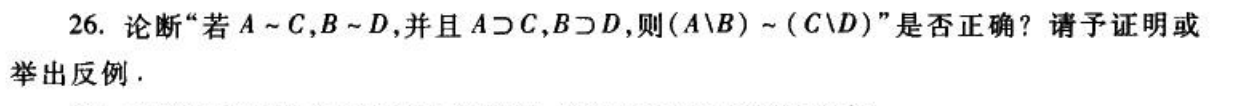
\includegraphics[width=\textwidth]{7-hw1-20250307.png}
% \caption{}
\label{}
\end{figure}

原题有误,$C\supset A, B\supset D$ 应改为 $A\supset B,C\supset D$.

$(A\setminus B)\sim(C\setminus D)$ does not always hold. A conterexample is as follow.

Let $A,B,C,D$ be groups, $B$ is a subgroup of $A$ and $D$ is a subgroup of $C$. The relation $\sim$ on groups is defined to be group isomorphism. Then we have $A\cong C$ and $B\cong D$. Since $\setminus$ is set minus, $A\setminus B$ or $C\setminus D$ is not a group! (without the identity) Therefore $(A\setminus B)\not\sim (C\setminus D)$.
